% !TEX root = ../../thesis.tex

\newpage
\section{Experimental evaluation of the role of the morphology: the thigh shape} % (fold)
\label{sec:morphology-role}

\subsection{Motivations} % (fold)

The role of morphology in robot biped locomotion has been particularly explored through the research on passive dynamic walkers~\cite{wisse2007passive}. The most famous example concerns the Tad MacGeer's work~\cite{mcgeer1990passive}. Thanks to the understanding of the intrinsic dynamics of its structure, McGeer has managed to create a 2D biped robot capable of producing several steps without any controller or motor.
The only control of this robot is obtained through the interaction between the intrinsic inertia of the structure and gravity.
This work has been pursued with the apparition of semi-passive walker combining both specific passive properties and low power actuation to increase their robustness~\cite{Anderson2005}. We can note the work of Collins~\cite{collins2005bipedal} which explored the case of semi-passive 3D biped robot. Its morphology is based on particular mass distribution, knee locking, round feet and springs on the legs to generate an efficient walking gait while keeping its lateral and frontal balance.
The concept of 3D semi-passive robot has been pushed even further with the realization of a complete humanoid robot with trunk, arms and head: the robot Denise~\cite{wisse2005three} and Flame presented in~\cite{Hobbelen2008}.

The geometry and distribution of mass in the body has complex influences on biped locomotion. Several studies have for example explored the role of the foot and ankle morphology for biped walking on both human~\cite{Adamczyk2006}~\cite{Hughes1990} and robot~\cite{hobbelen2005ankle}~\cite{Davis2010} However, to our best knowledge no research has focused on the role of the thigh for biped locomotion.  A few robots like HRP-4C~\cite{kaneko2009cybernetic} and Kenshiro humanoid~\cite{nakanishi2013design} robots seem to visually have a morphology design close to the thigh shape of Poppy, but no comparative study of the role of this shape was presented so far.

Thanks to the conception of Poppy allowing easy, cheap and fast morphology modifications, we are able to experiment the impact of various thigh shapes on the robot dynamics. In particular, in this experiment, we will focus on its bio-inspired thigh shape, bended by an angle of 6\textsuperscript{o}. We will investigate the impact of this thigh design on the balance and biped locomotion using a comparison with a more traditional straight thigh (see Fig.~\ref{fig:poppy_compared}).

% The results presented in the incoming sections have been published in the Humanoids 2013 conference proceeding~\cite{lapeyre:hal-00861110}.


\begin{figure}[!t]
\centering
    \subfloat[][bended thighs]{\label{fig:poppy_with_bended_legs}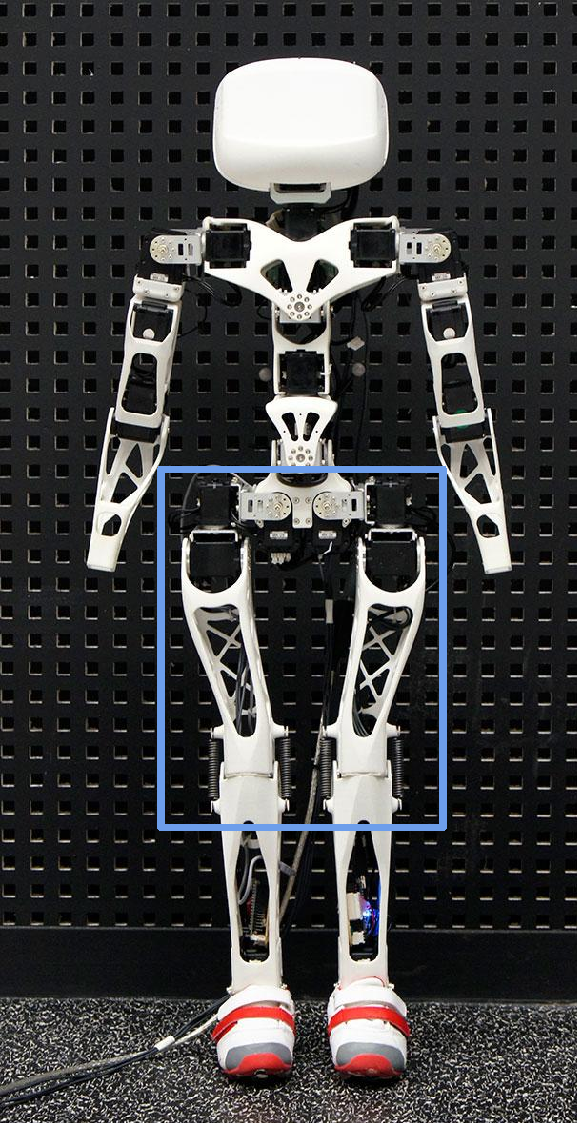
\includegraphics[width=0.35\linewidth]{poppy_bended_tigh_square.pdf}}
    \hfil
    \subfloat[][straight thighs]{\label{fig:poppy_with_classical_legs}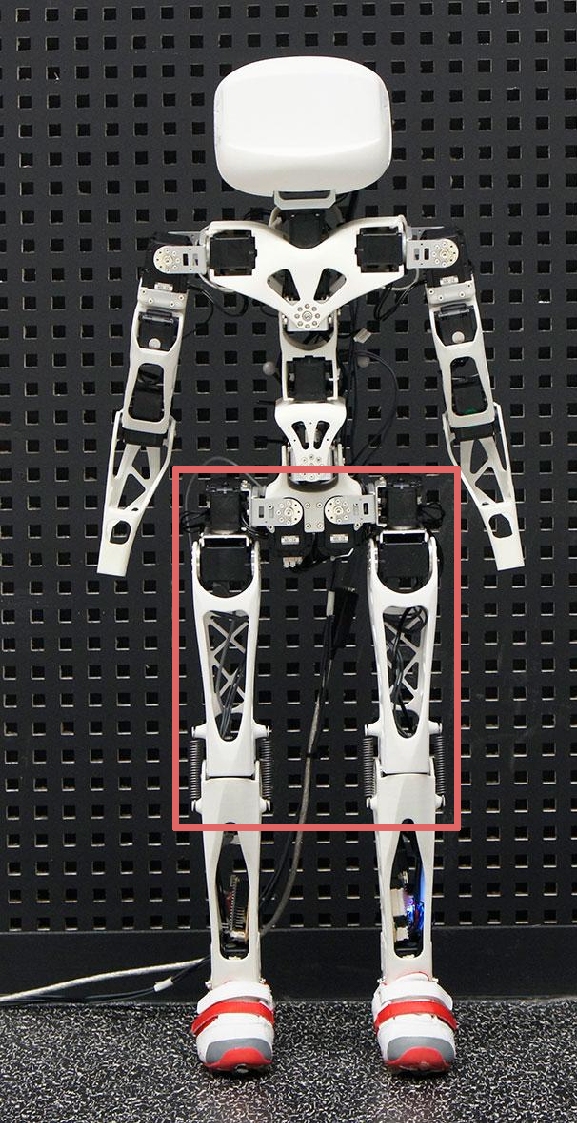
\includegraphics[width=0.35\linewidth]{poppy_straight_tigh_square.pdf}}
    \caption{We evaluate the effect of the thigh morphology on the biped locomotion dynamic.
    Experiments are made using the Poppy humanoid platform.
    In this paper, we compare two thigh morphologies: (a) thigh bended by an angle of 6\textsuperscript{o} and (b) a more classical approach with straight thighs.}
    \label{fig:poppy_compared}
\end{figure}


\subsection{Understanding the role of the thigh shape in human} % (fold)

If we look closely at the human's femur morphology, it appears that it is inclined by an angle of 6\textsuperscript{o}. This makes the feet closer to the projection of the center of gravity (see Fig.~\ref{fig:human_thigh}) and leads to two main stability enhancements during the walking gait:

\begin{itemize}
    \item As the feet are closer to the gravity center, the necessary lateral translation of the CoG to transfer the mass of the robot from one foot to another is reduced (see Fig~\ref{fig:human_thigh}). In the case of Poppy's morphology, thanks to the $6$\textsuperscript{o} bended thigh, the lateral motion of the CoG is reduced by about 30\% ($ 5 cm$ instead of $7.1 cm$).
    \item During the stance phase, the CoG initial conditions are slighty modified. As we will explain with a simple theoritical model in the next section, the bended thigh can reduce the falling rate.
\end{itemize}


\begin{figure}
\centering
    \subfloat[][]{\label{fig:human_thigh}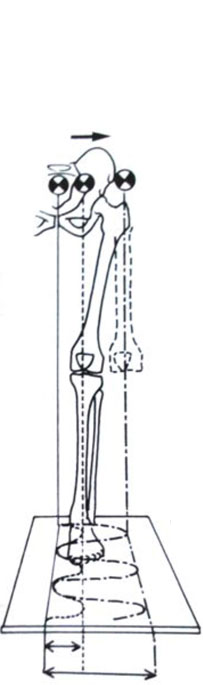
\includegraphics[height=8cm]{human_thigh.jpg}}
    \hfil
    \subfloat[][]{\label{fig:model_thigh}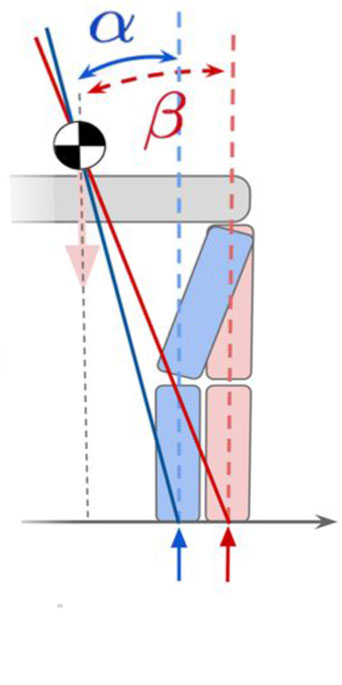
\includegraphics[height=8cm]{model_thigh.jpg}}
    \hfil
    \subfloat[][]{\label{fig:thigh_of_poppy}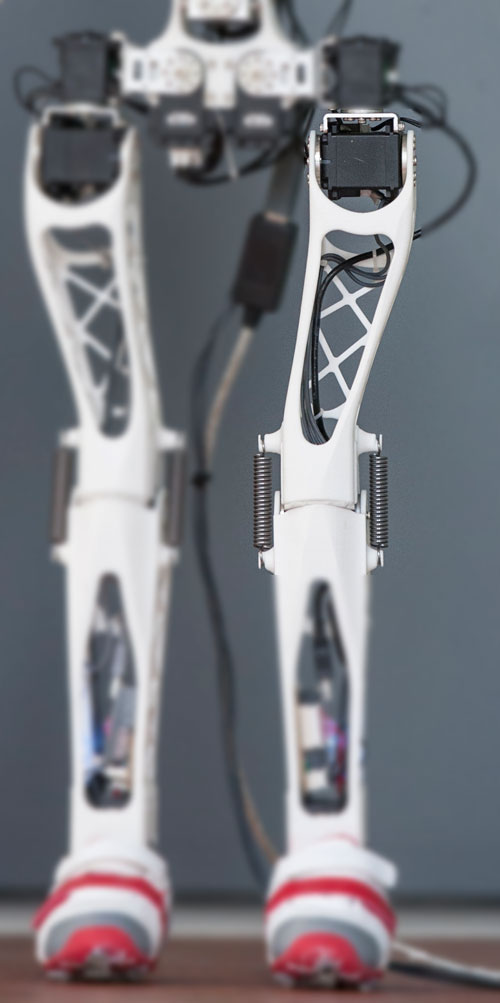
\includegraphics[height=6cm]{thigh_shape_large.jpg}}
    \caption{ a) Effect of the human being bended femur on the human biped locomotion.
    b) Model used for the comparison of the two thighs morphology.
    c) Actual realization of the bended thigh on the poppy platform}
    \label{fig:poppy_thigh}
\end{figure}

\subsubsection{Theoretical model} % (fold)
\label{sub:exp_theoritical_model}

We can model the situation where the robot is on one foot by an inverted pendulum with a point mass centered on the center of gravity (CoG) of the robot and the axis of rotation located at the foot position (see Fig.~\ref{fig:thigh_of_poppy}). With such model, the dynamic of the whole structure depends on:

\begin{itemize}
    \item the length $l$ of the segment extending from the foot to the center of gravity,
    \item the angle $\theta$ of the segment relative to the vertical,
    \item the gravity force $g$.
\end{itemize}

And the system follows this physical law:

\begin{equation}
    \ddot{\theta}(t) + w_0 \cdot sin(\theta(t)) = 0
\end{equation}
with:
\begin{equation}
    w_0 = \sqrt{\frac{g}{l}}
\end{equation}

\subsubsection{Intuitive expectation} % (fold)

To get a first insight of the behavior, we can linearize the system for small disturbance such as:

\begin{equation}
    \theta(t) = \theta_0 \cdot cos(w_0\cdot t)
\end{equation}
and
\begin{equation}
    \dot{\theta}(t) = -\theta_0 \cdot w_0 \cdot sin(w_0\cdot t)
\end{equation}

One can notice the position and velocity of the pendulum linearly varies with the initial condition i.e $\theta$ angle. Thus reducing this initial angle $\theta_0$ involves a direct reduction of the falling speed $\dot{\theta}(t)$ of the robot.

In the case of Poppy's geometry, the thigh bending allows a 40\% reduction of the initial angle $\theta_0$ ($\alpha = 3.8$\textsuperscript{o} against $ \beta = 6.4$\textsuperscript{o} on Fig.~\ref{fig:model_thigh}).

\subsubsection{Simulation} % (fold)

In the case of a fall, it is not possible to make the assumption of small perturbations, that is the reason why we have simulated the model in Matlab with a non-linear system and obtain the behavior represented in Fig.~\ref{fig:dynamic_thigh_model}.

\begin{figure}[thpb]
    \centering
    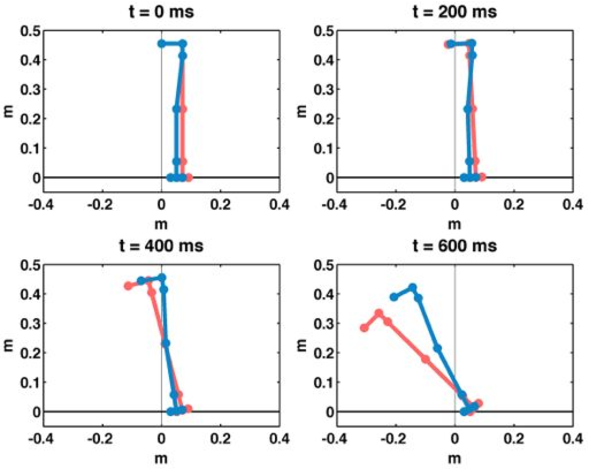
\includegraphics[width=0.8\linewidth]{dynamic_thigh_model.pdf}
    \caption{Comparison of the falling dynamic over time when Poppy is standing on one foot depending on  its thigh morphology: with a bended thigh of 6\textsuperscript{o} (blue) and with a straight thigh (red).}
    \label{fig:dynamic_thigh_model}
\end{figure}

If we define the center of gravity altitude as:
\begin{equation}
    z_{CoG} = l \cdot cos(\theta(t))
\end{equation}
We can express its falling speed over time as:
\begin{equation}
    \dot{z}_{CoG} = - \dot{\theta}(t) \cdot l \cdot sin(\theta(t))
\end{equation}

In this condition, if we consider the first 700ms of the system behavior simulation and compare the two systems, the mean of the CoG falling speed is reduced by around 56\% in the bended thigh case.


\subsection{Experimenting thigh properties variation with Poppy} % (fold)

The simple model described in the previous section showed that a slight inclination (6\textsuperscript{o}) of the thigh can theoretically have a significant gain regarding the lateral stability of the robot during the two main phases of the walking gait (i.e. single stance phase and double stance phase).

In this section, we describe representative experiments which evaluate the actual gain of the thigh shape on the real Poppy platform. To do this, we used both a pair of straight thighs and the bended thighs presented above. We will compare Poppy's reactions with those different legs (see Fig.~\ref{fig:poppy_compared}) on three experiments:
\begin{itemize}
    \item Evaluate the falling speed during single support stance.
    \item Measure the lateral translation to move the CoG Form one feet to the other.
    \item Record the upper body motion during biped locomotion.
\end{itemize}

\subsubsection{Single support falling velocity} % (fold)
\label{ssub:falling_velocity}
The experiment evaluates the fall velocity of Poppy when it is supported on only one foot and compare it with the theoretical results obtained in~\ref{sub:exp_theoritical_model}. To do so, the robot's head is tracked by an Optitrack\footnote{\url{http://www.naturalpoint.com/optitrack/products/v120-trio/}} device and markers are placed on the head. In postural balance on two feet, a motor order triggers the raise of a foot which unbalances the robot (see Fig.~\ref{fig:falling_experiment_dispositif}) and causes its lateral fall (see Fig.~\ref{fig:fall_of_poppy}). This experiment was repeated about fifteen times for the two cases studied, i.e. with bended legs (Fig.~\ref{fig:poppy_with_bended_legs}) and with straight legs (Fig.~\ref{fig:poppy_with_classical_legs}).

\begin{figure}[h]
\centering
    \subfloat[][]{\label{fig:falling_experiment_dispositif}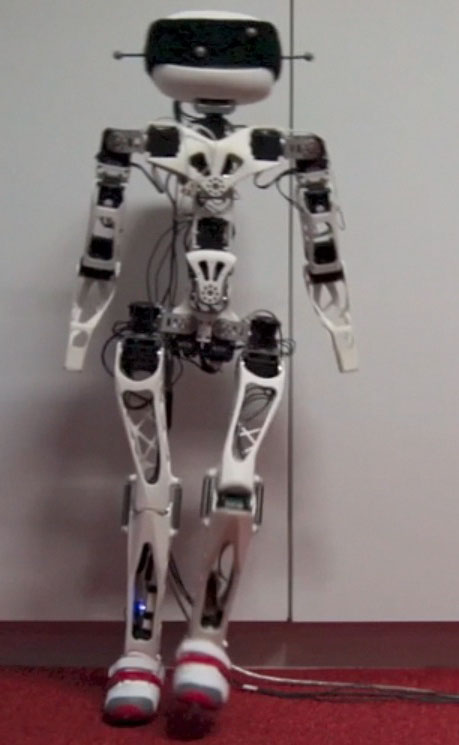
\includegraphics[height=6cm]{experience_fall_illu.jpg}}
    \hfil
    \subfloat[][]{\label{fig:fall_of_poppy}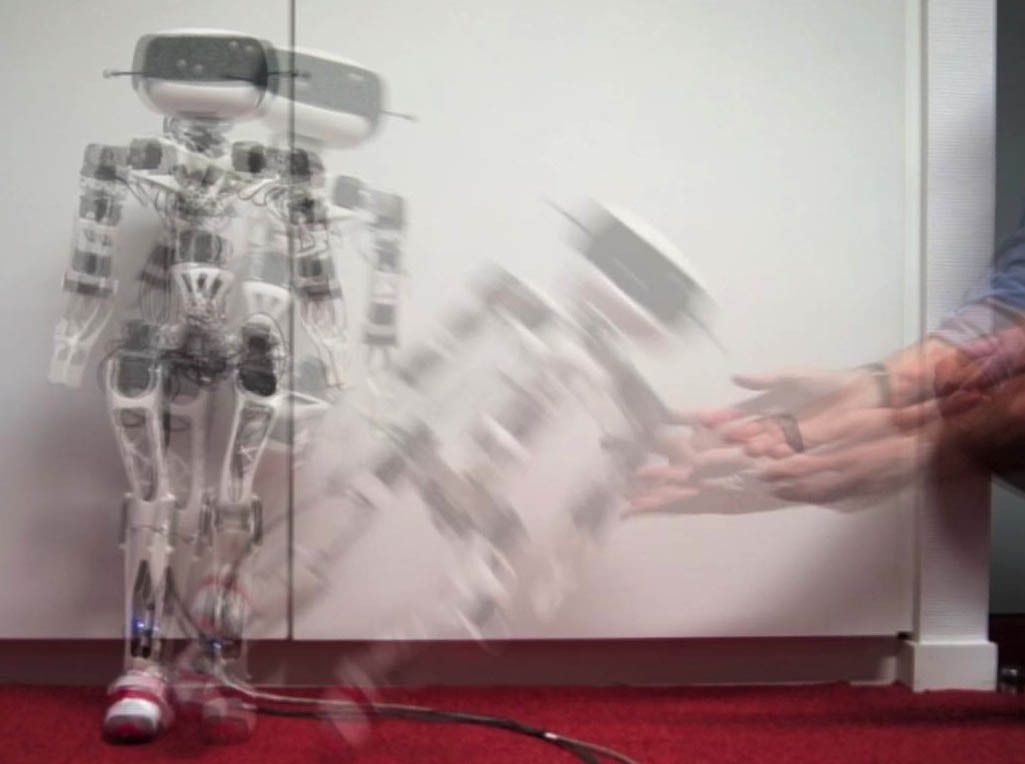
\includegraphics[height=6cm]{experience_fall_mean.jpg}}
    \caption{Run of the one support stance falling experiment.
    The Poppy head has a headband with markers to track its absolute position over time.
     a) Initial perturbation done a sudden raise of one foot, b) view of the Poppy lateral fall over time.}
    \label{fig:falling_experiment}
\end{figure}

Experiments results are shown on the Fig.~\ref{fig:falling_results}. The blue color is assigned to experiments with bended thighs while the red color is assigned to straight thighs. For each case, the light color corresponds to the standard deviation and the dark color to the 95\% confidence interval of the mean value. The first figure~(\ref{fig:fall_result_position}) refers to the head altitude position over time and the second~(\ref{fig:fall_result_velocity}) to the falling velocity of the head. Dashed lines represent theoretical results obtained with the model presented in section~\ref{fig:model_thigh}. One can notice the strong similarity both on the shape and on the difference between the two morphologies studied. Yet, there is a slight time shift between theoretical and experimental results. This can be explained by the inertia of the real robot which was not took into account during the simulation.

\begin{figure}[h]
\centering
    \subfloat[][Vertical head position]{\label{fig:fall_result_position}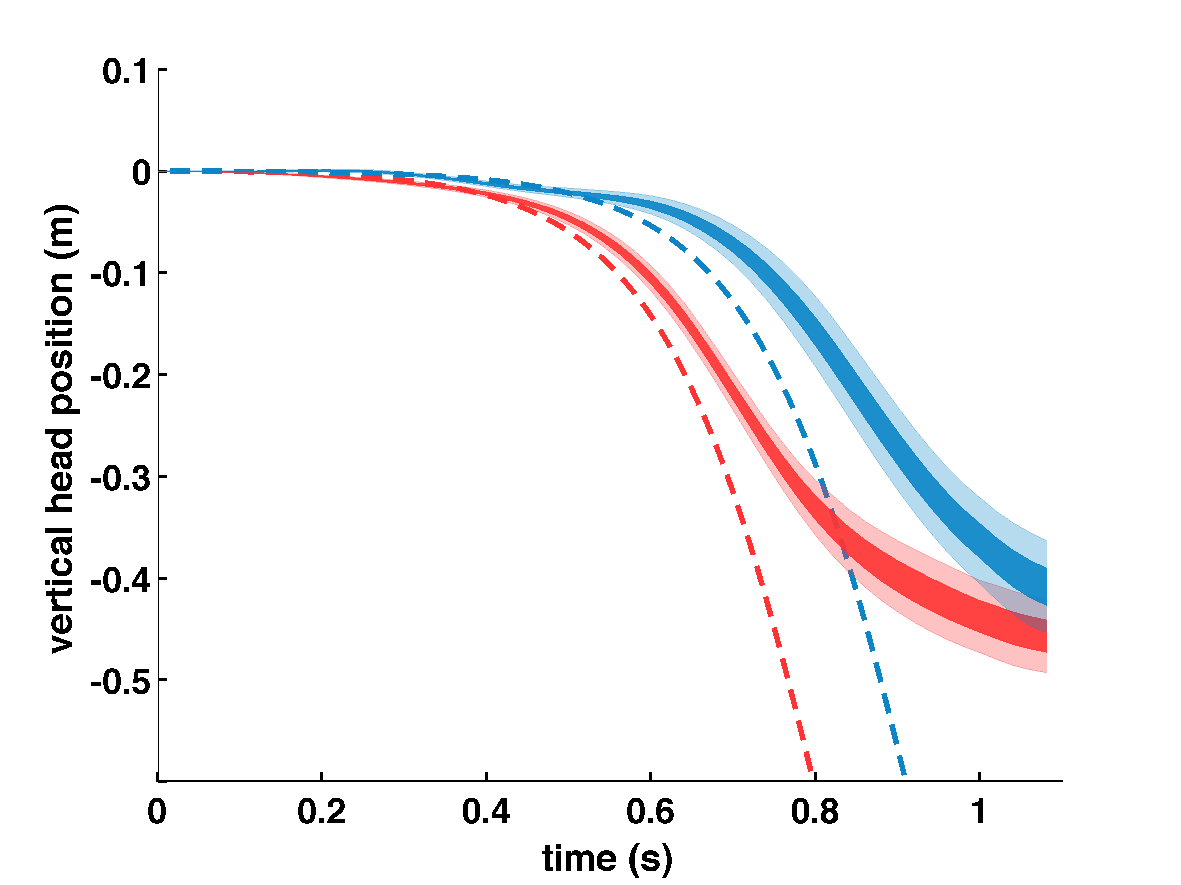
\includegraphics[width=0.50\linewidth]{falling_compare.pdf}}
    \hfil
    \subfloat[][Vertical head falling velocity]{\label{fig:fall_result_velocity}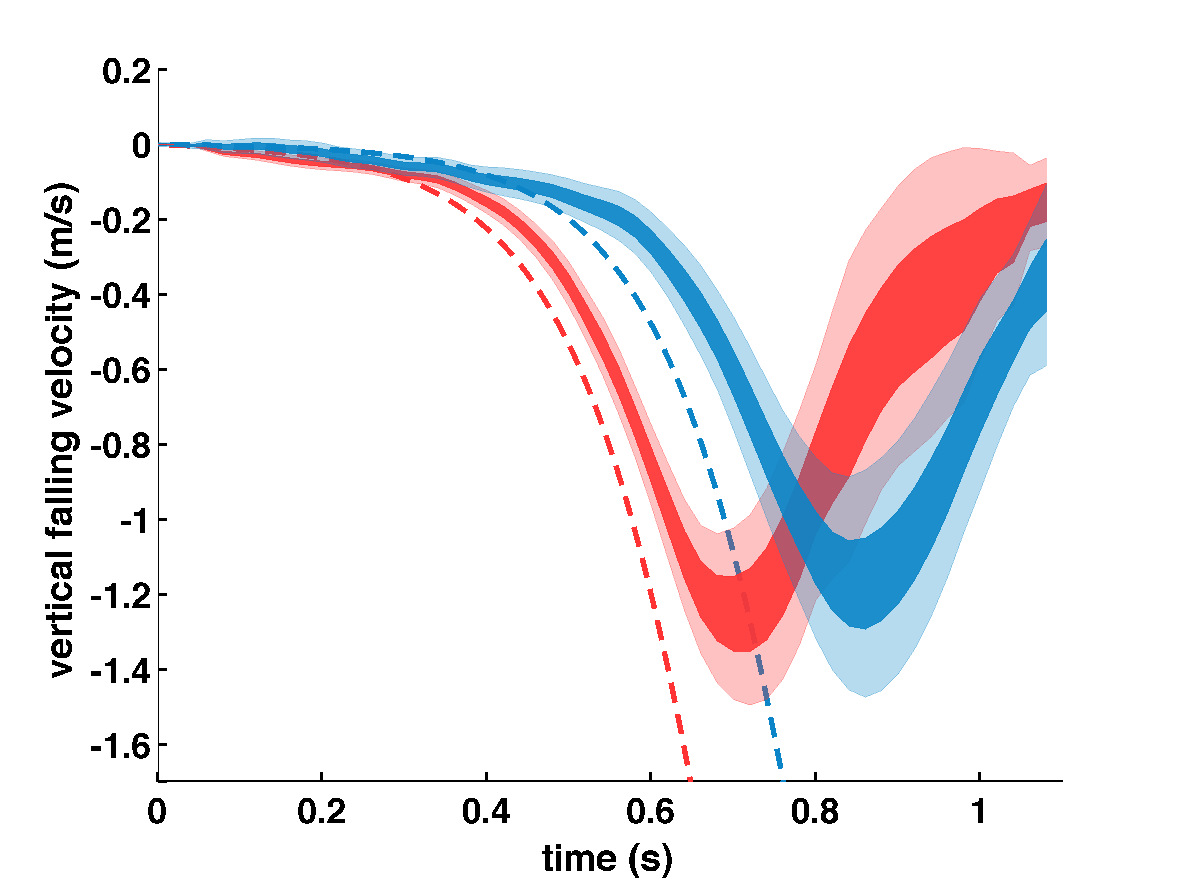
\includegraphics[width=0.50\linewidth]{velocity_compare.pdf}}
    \caption{Results of the single support falling experiment.
    The blue color is associated with experiments conducted with bended thighs while the red color is assigned to straight thighs.
    For each case, the light color corresponds to the standard deviation and the dark color to the 95\% confidence interval of the mean value while dashed lines represent theoretical results.
    These figures shows the vertical position (a) and vertical falling velocity (b) of the head of Poppy over time for each case studied.
    The curves behavior change after 800ms is due to the fact that we catch up the robot before it touches the ground.}
    \label{fig:falling_results}
\end{figure}

These figures show a clear improvement for the Poppy version with bended thigh (blue curves) with a 200ms time shift compared to the straight thigh (as illustrated on the attached video\footnote{\url{http://flowers.inria.fr/Humanoid2013/}\label{video}}).
Thanks to this delay, the falling speed is reduced by about 56\% during the first 700ms. Thus the robot remains almost stationary for 600 ms (400ms in the case of straight thigh). The typical walking gait of Poppy is done over a period of one second so the mono-pedal stance phase last around 420 ms~\cite{lapeyre2013poppy}. Considering that the robot remains stationary during more time than the single stance phase, we can imagine that the lateral balance control will be reduced during the walking gait.



\subsubsection{Double support CoG transfer} % (fold)
\label{sub:cog_motion}


In this experiment we evaluate the necessary lateral movement of the robot to cause a displacement of its center of gravity from one foot to the other and verify the theoretical results obtained previously. For this, Poppy is placed on a force platform to measure the displacement of its center of pressure. The absolute movements of the robot are tracked with an OptiTrack device and markers placed at the head and lower back (approximately the position of the actual center of gravity). The robot is kept rigid in a neutral position and a human physically pushed it from left to right until it reaches its lateral falling limit. As this operation is not very accurate, the experiment is repeated a hundred times.

\begin{table}[h]
\centering
\begin{tabular}{|l|c|c|c|}
  \hline &      Straight tigh &                     Bended Tigh &                   diff(\%) \\
  \hline CoP & 74.6 {\scriptsize$\pm$9.0} mm &     49.8 {\scriptsize$\pm$7.7} mm & 33\\
  Head & 100.1{\scriptsize$\pm$14.4} mm&     62.9{\scriptsize$\pm$22.0} mm &  37\\
  Lower Back & 64.1{\scriptsize$\pm$11.5} mm&      43.4{\scriptsize$\pm$15.0} mm &  32 \\
  \hline
\end{tabular}
\caption{Summary of the results obtained during the experiment on the lateral motion needed to transfer the robot mass from one foot to the other.}
\label{tab:CoG_motion}
\end{table}

The table~\ref{tab:CoG_motion} presents for each area considered (i.e. center of pressure (under feet), lower back and head motion) the amplitude of the lateral motion (in millimeter) needed to translate the CoG of the robot from one foot to the other for the two versions of the Poppy thigh design. The last columns summarizes the relative difference between the two conceptions (in percent). One can note that the results show a reduction of lateral movement of around 30\%. Thanks to the shape of the thigh, the lateral displacement of the upper body required to move the CoG from one foot to the other can be reduced.


The results presented on the two first experiments show improvement for two main aspects needed during biped locomotion: lateral stability and mass transfer. In the next experiment, we will evaluate if there is a significant performance gain in a complex dynamic phase such as bipedal walking.


\subsubsection{Walking dynamic} % (fold)
\label{sub:walking_dynamic}

As explained in the introduction and description of the platform, Poppy has been especially designed to study bipedal walking and human-robot interaction.

Here the experiment consists in playing an open-loop walking pattern while the robot is guided through the physical interaction with a human. The users role is to provide both balance and control of mass transfer. By producing small lateral motion on the upper-body they can help the robot to move its CoG from one foot to another.

\begin{figure}[h]
    \centering
    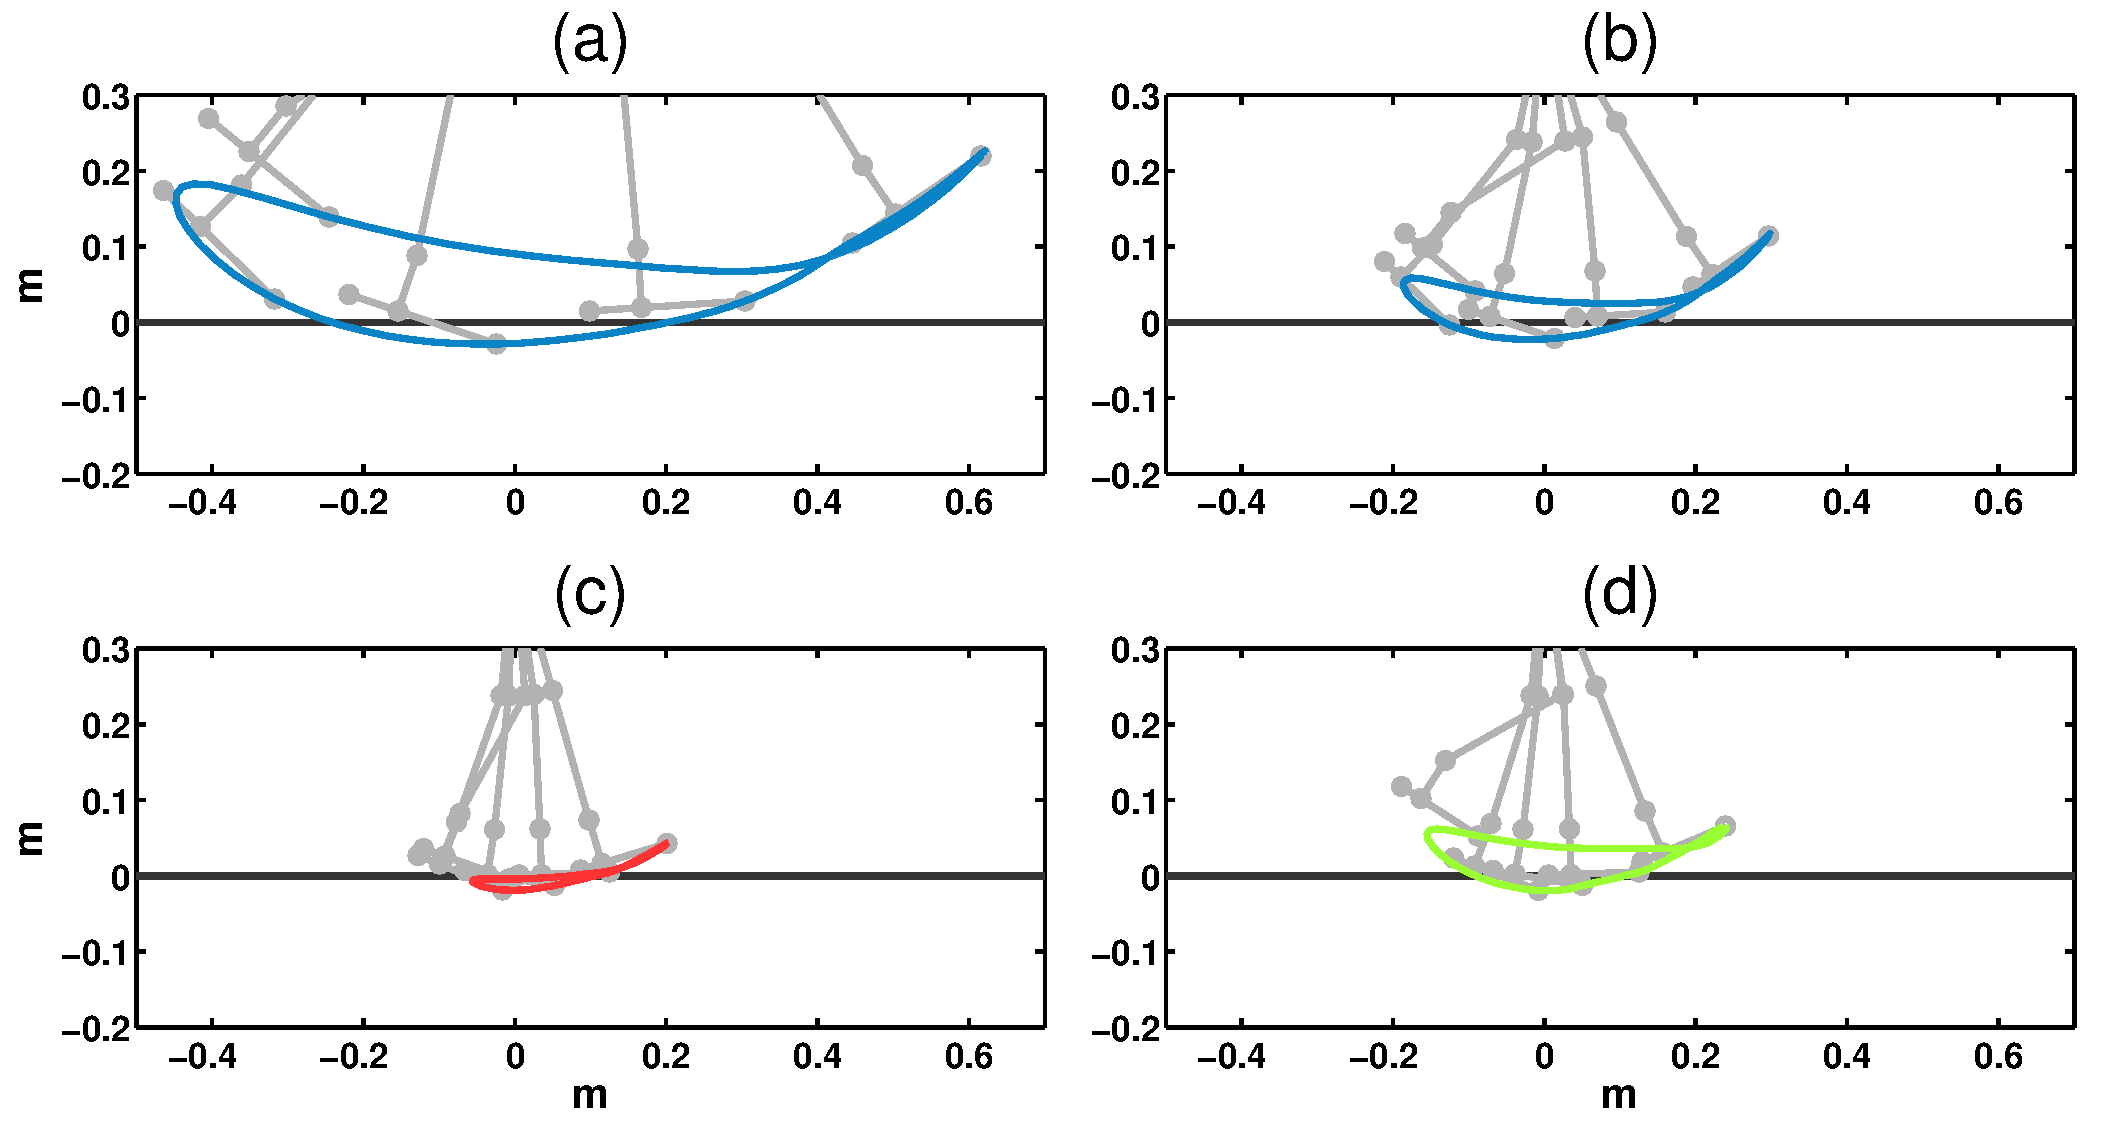
\includegraphics[width=0.95\linewidth]{CPG.pdf}
    \caption{Toes trajectories generated by the walking pattern a) Kinematics of human walking
    with human's morphology b) Direct transposition of the human kinematics with Poppy's morphology
    c) Reducing amplitude of the human kinematics joints with Poppy's morphology d) Walking pattern
    used for the experiment with Poppy}
    \label{fig:CPG}
\end{figure}

The gait is based on the actual human sagittal joint kinematic~\cite{Nester2003}: hip, knee, ankle (see Fig.~\ref{fig:CPG}.a). A direct transposition of the human joint kinematic on the Poppy's morphology results in a walking speed which is too fast to be handled by users (see Fig.~\ref{fig:CPG}.b). A simple reduction of joints amplitude conducts to an unsuitable leg trajectory where toes bump into the ground during the swing phase (see Fig.~\ref{fig:CPG}.c). So to ensure enough clearance during the swing phase and suitable walking speed for the guidance with user, we modified the joints trajectories by hand to both reduce the length step and increase the foot clearance (see Fig.~\ref{fig:CPG}.d). The actual gait on Poppy is shown on the Fig.~\ref{fig:humanoids2013_cpg_on_poppy}.

\begin{figure}[h]
    \centering
    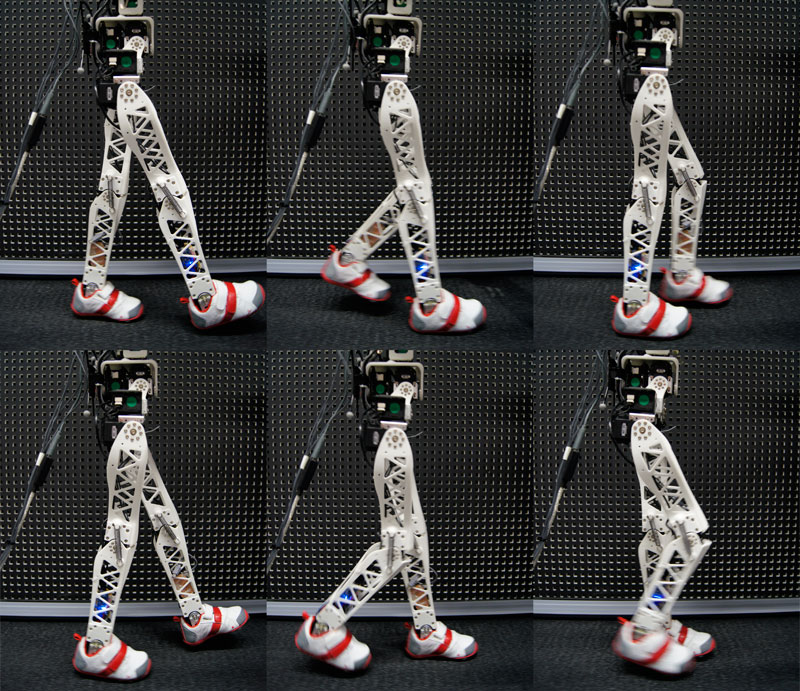
\includegraphics[width=0.9\linewidth]{walking_poppy.jpg}
    \caption{Walking gait CPG described on Fig.~\ref{fig:CPG}.d applied on the actual Poppy robot.
    The CPG generates a human-like walking gait allowing the robot to walk at 1.8km/h and involves straight leg during the stance phase.
    There is no balance control but stability is obtained through physical guidance with trained expert user.}
    \label{fig:humanoids2013_cpg_on_poppy}
\end{figure}

In this experiment we are interested by the dynamic of Poppy especially on the frontal plane and we will compare the effect of the thigh shape on this dynamic. Poppy walks on a treadmill following the walking gait described above. An expert user trained to keep the robot in the correct walking cycle provides guidance to the robot. This is done by keeping the robot in a vertical position and supporting, in a compliant manner, the lateral movement of the robot as illustrated in attached videos. The user is asked to do the best he can to minimize the movement/forces he applies in both morphologies to reduce the bias towards the two design experimented. All proprioceptive sensors are recorded at 50hz while an Optitrack device associated to markers located at the head and lower back measure the absolute displacements of the robot (voir Fig.~\ref{fig:walking_experiment}).

\begin{figure}[!h]
    \centering
    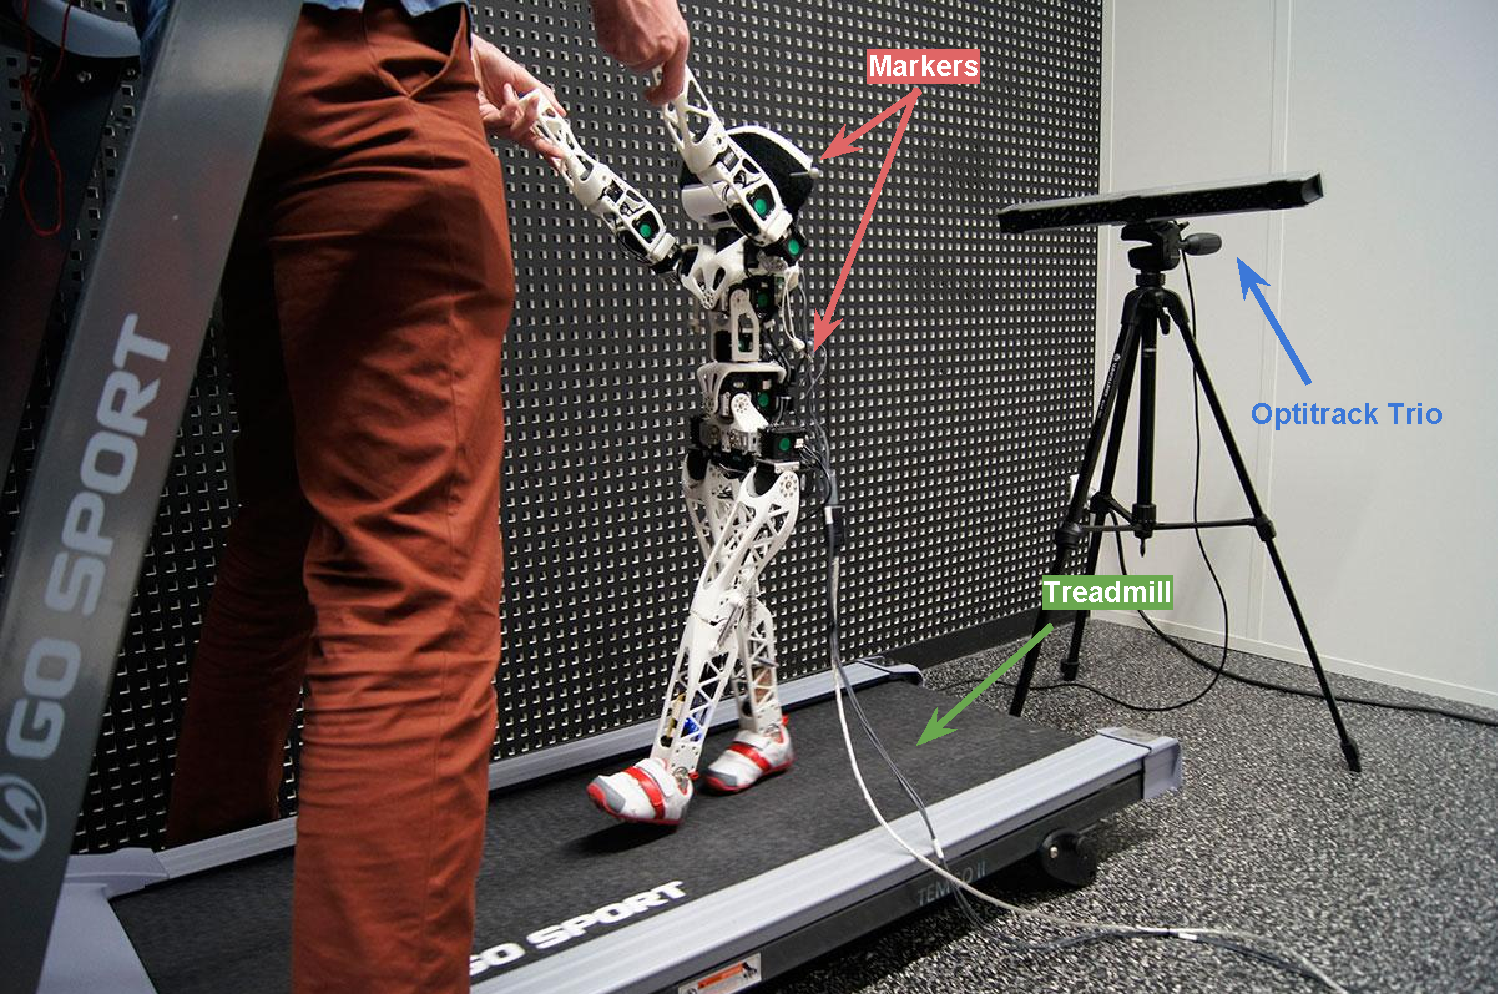
\includegraphics[width=0.8\linewidth]{dispositif_experience_marche.pdf}
    \caption{Proceeding of the walking experiment.
    Poppy is tracked by an Optitrack trio while it is walking on a treadmill set at 1.8km/h.
    An expert user provides the sagittal balance needed during all the experiment.}
    \label{fig:walking_experiment}
\end{figure}

The Poppy dynamic is recorded for around 1800 walking gait cycle for each thigh design (around 90,000 data points for each case). Data are folded over to extract the gait behavior over a gait cycle. Results are presented on Fig.~\ref{fig:walk_result}. As previously, the blue color is assigned to experiments with bended thigh, the red color is assigned to straight thigh. For each case, the light color corresponds to the standard deviation and the dark color to the 95\% confidence interval of the mean value.

\begin{figure}[!h]
    \subfloat[][Lateral head displacement]{\label{fig:head_position}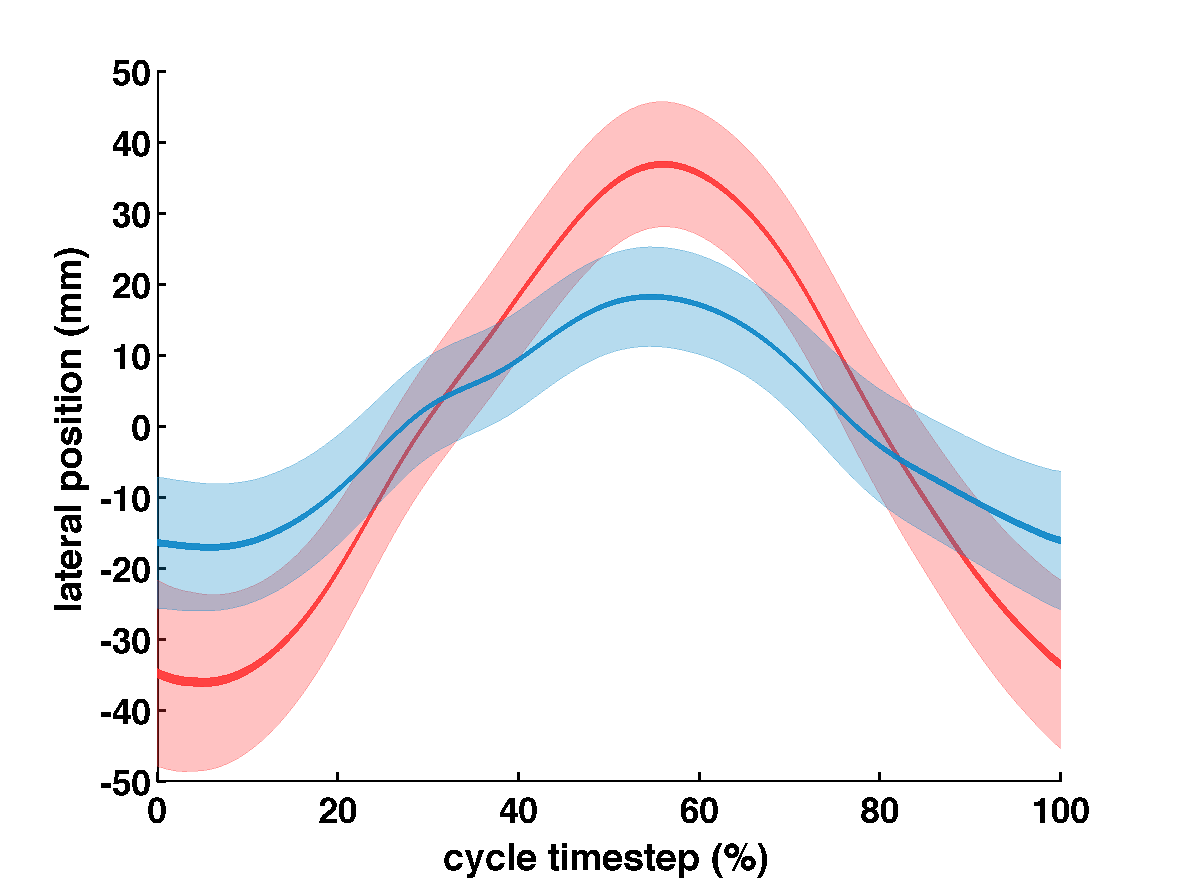
\includegraphics[width=0.49\linewidth]{marche_head_motion.pdf}}
    \hfil
    \subfloat[][Lateral lower back displacement]{\label{fig:low_back_position}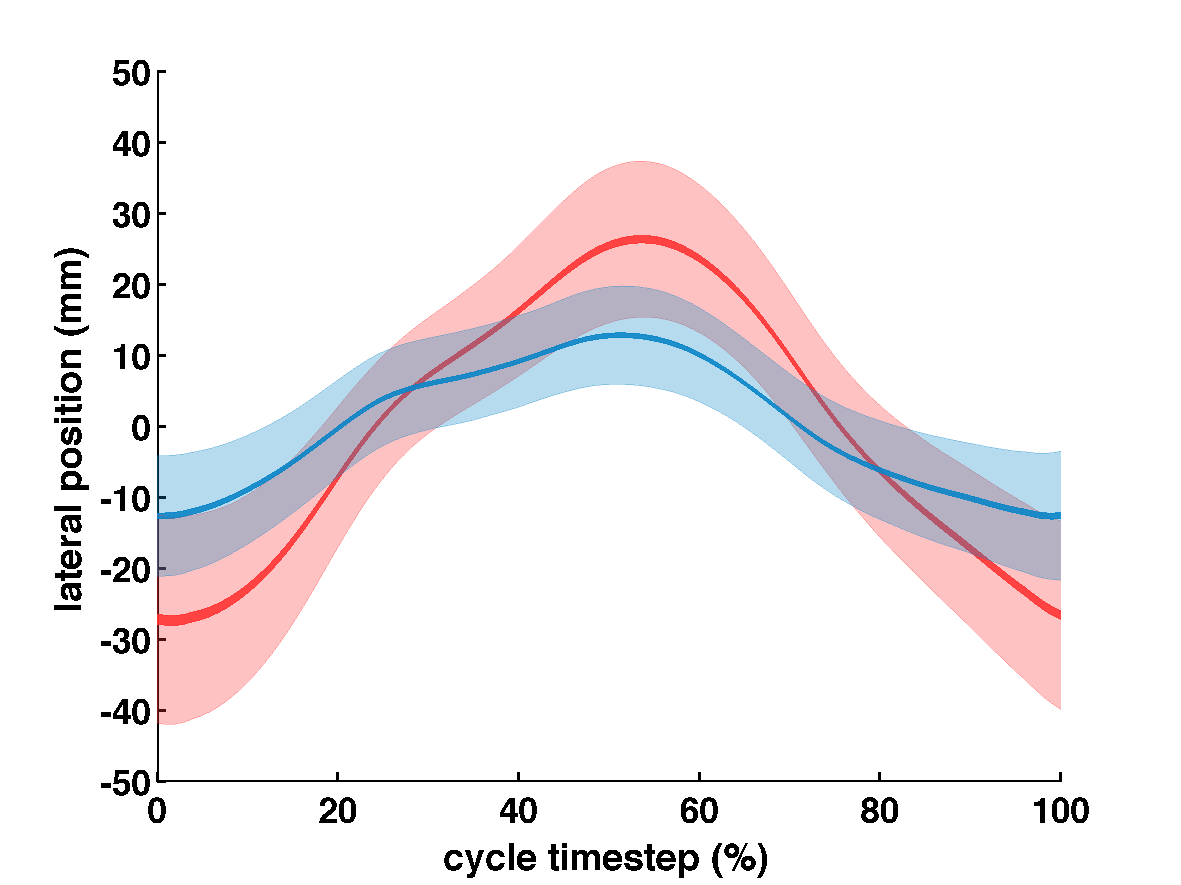
\includegraphics[width=0.49\linewidth]{marche_low_back_motion.pdf}}
    \hfil
    \subfloat[][Sagittal head acceleration]{\label{fig:head_acceleration_x}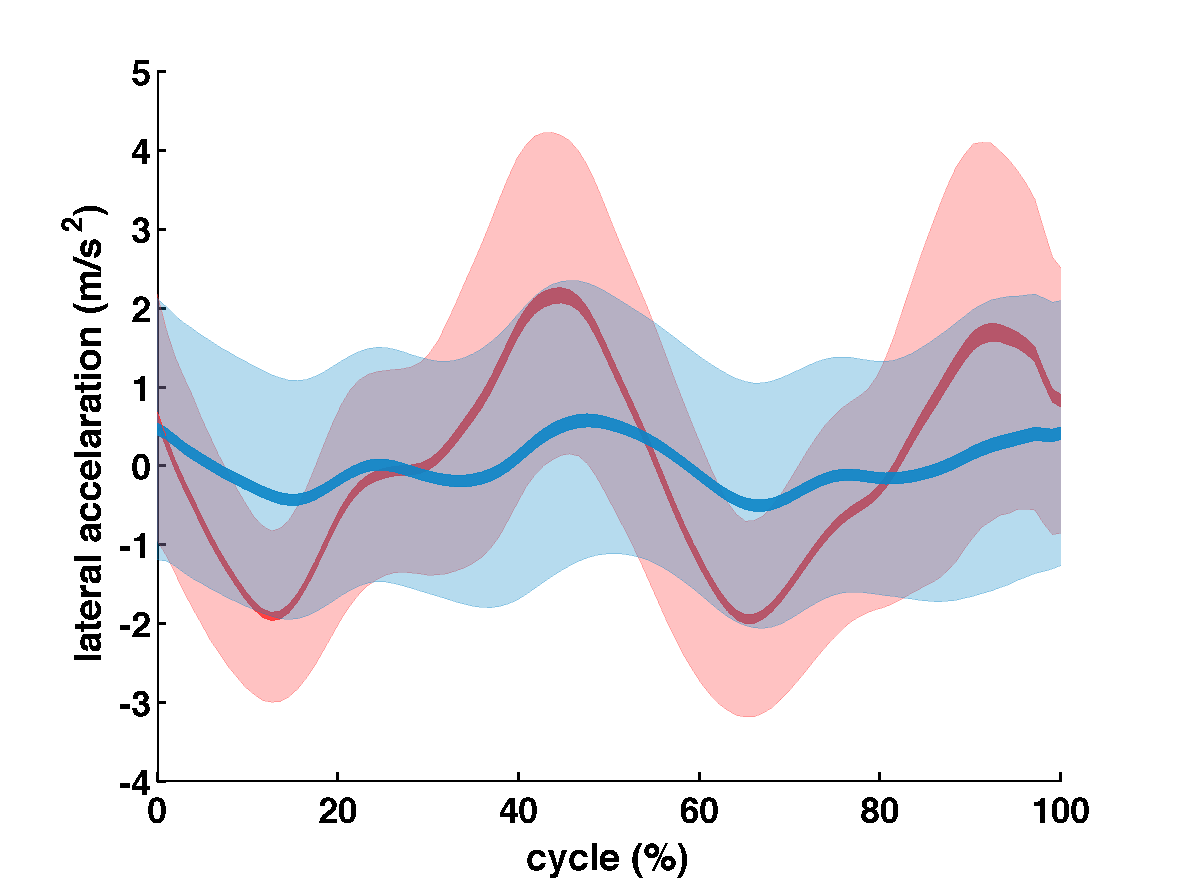
\includegraphics[width=0.49\linewidth]{marche_accel_x_signal.pdf}}
    \hfil
    \subfloat[][Lateral head acceleration]{\label{fig:head_acceleration_y}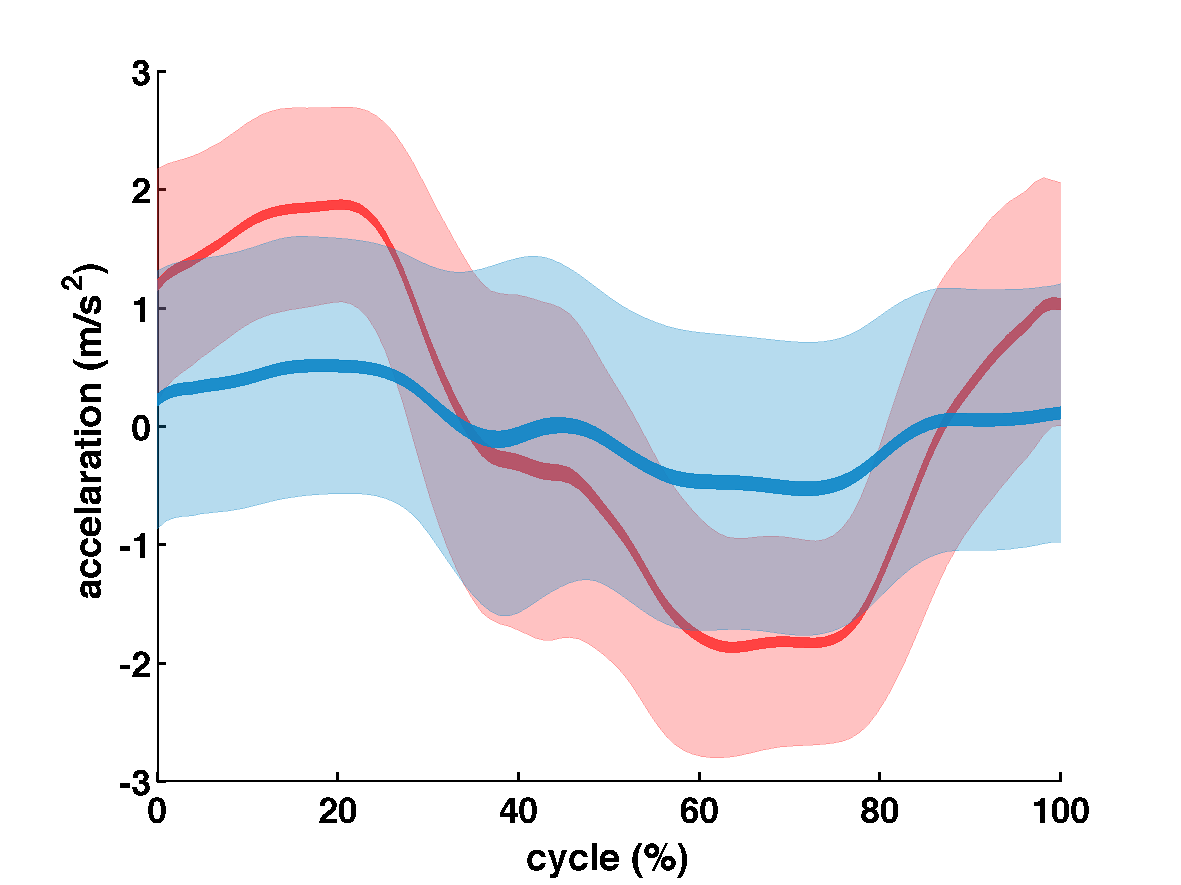
\includegraphics[width=0.49\linewidth]{marche_accel_y_signal.pdf}}
    \hfil
    \subfloat[][Speed of rotation in the frontal plane]{\label{fig:head_gyro_x}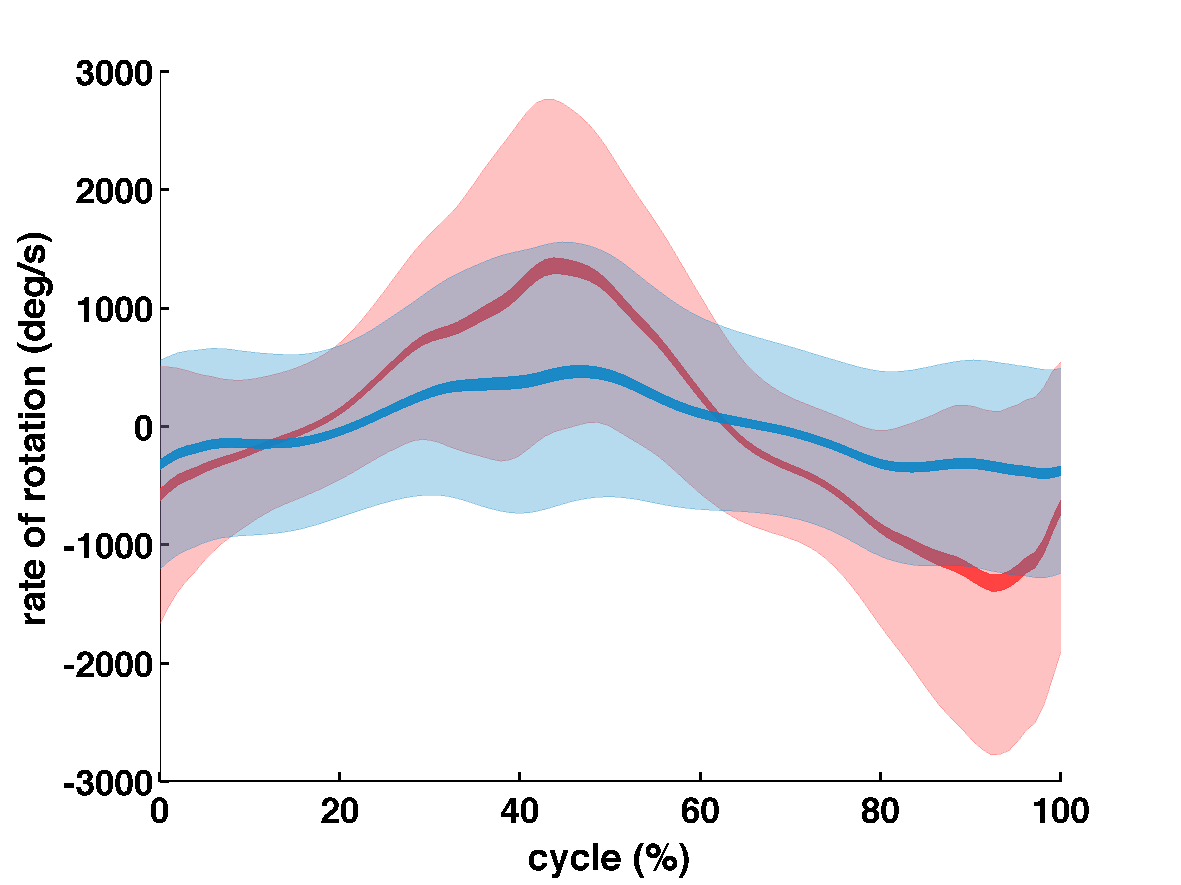
\includegraphics[width=0.49\linewidth]{marche_tilt_x_signal.pdf}}
    \hfil
    \subfloat[][Head inclinaison]{\label{fig:head_tilt_x}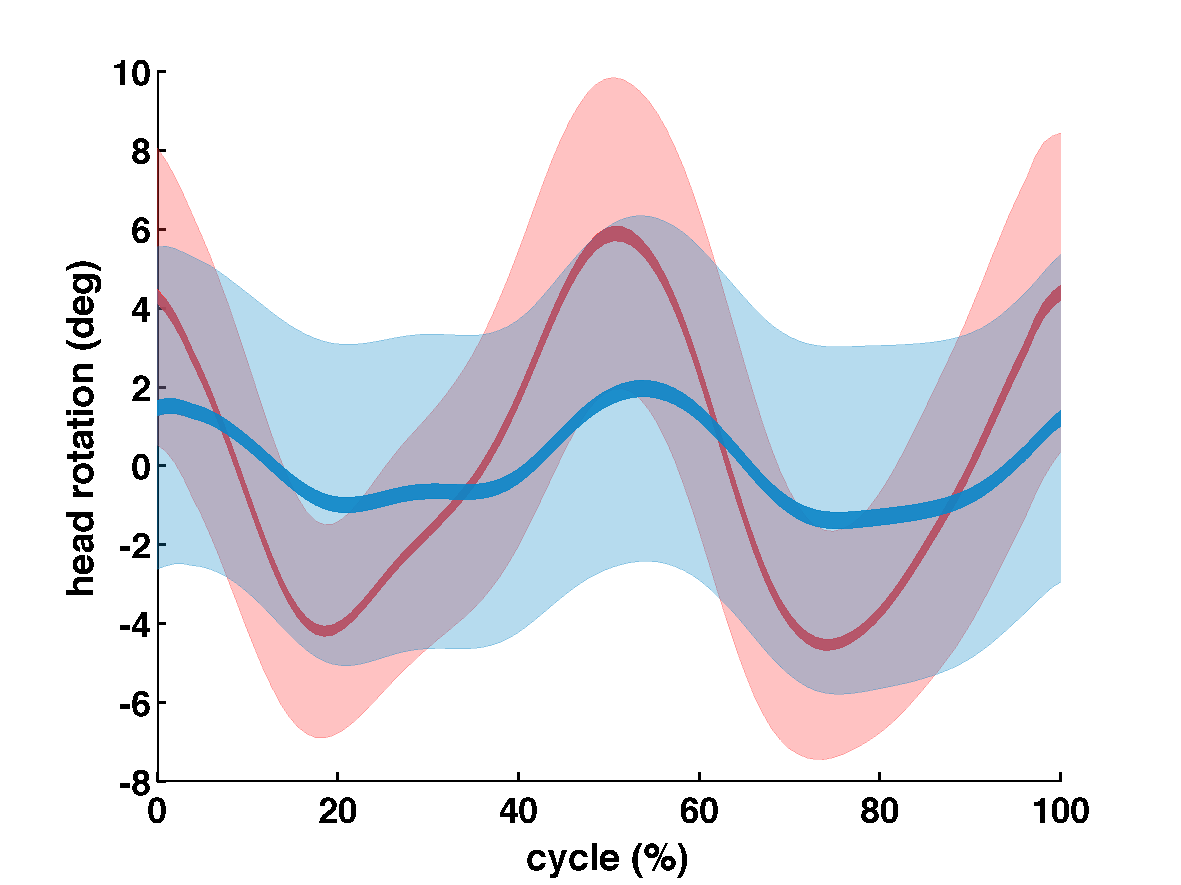
\includegraphics[width=0.49\linewidth]{marche_tilt_y_signal.pdf}}
    \caption{Results obtained during the walking experiment.
    The blue color is associated with experiments conducted with bended thighs while the red color is assigned to straight thighs.
    For each case, the light color corresponds to the standard deviation and the dark color to the 95\% confidence interval of the mean value.
    All data are folded over to extract the mean gait behavior and its standard deviation over a walking gait cycle expressed in percent.}
    \label{fig:walk_result}
\end{figure}

The two first figures (i.e. ~\ref{fig:head_position} and ~\ref{fig:low_back_position}) show the upper body lateral motion in millimeter over the gait cycle. We can notice that for the two designs, the motion pattern shown by the upper body (head and lower back) is similar. However in the case of the bended thigh (blue) the amplitude of the motion is reduced by about 45\%. Another interesting effect concerns the head perturbations shown on figures ~\ref{fig:head_acceleration_x}, and ~\ref{fig:head_acceleration_y}. Here also, patterns are similar but in the case of the bended thigh the head is clearly less perturbed by the walking dynamic with a reduction in amplitude of approximately 30\%. Five pictures have been taken while Poppy was walking and were stacked on Fig.~\ref{fig:poppy_walking_compared}. This shows a qualitative point of view of the walking dynamic for both studied case.
We can notice that the lateral motion of the version of Poppy with bended thigh~\ref{fig:poppy_walking_bended} is small compared to the version with straight thigh~\ref{fig:poppy_walking_straight}.


\begin{figure}[h]
\centering
    \subfloat[][bended thigh]{\label{fig:poppy_walking_bended}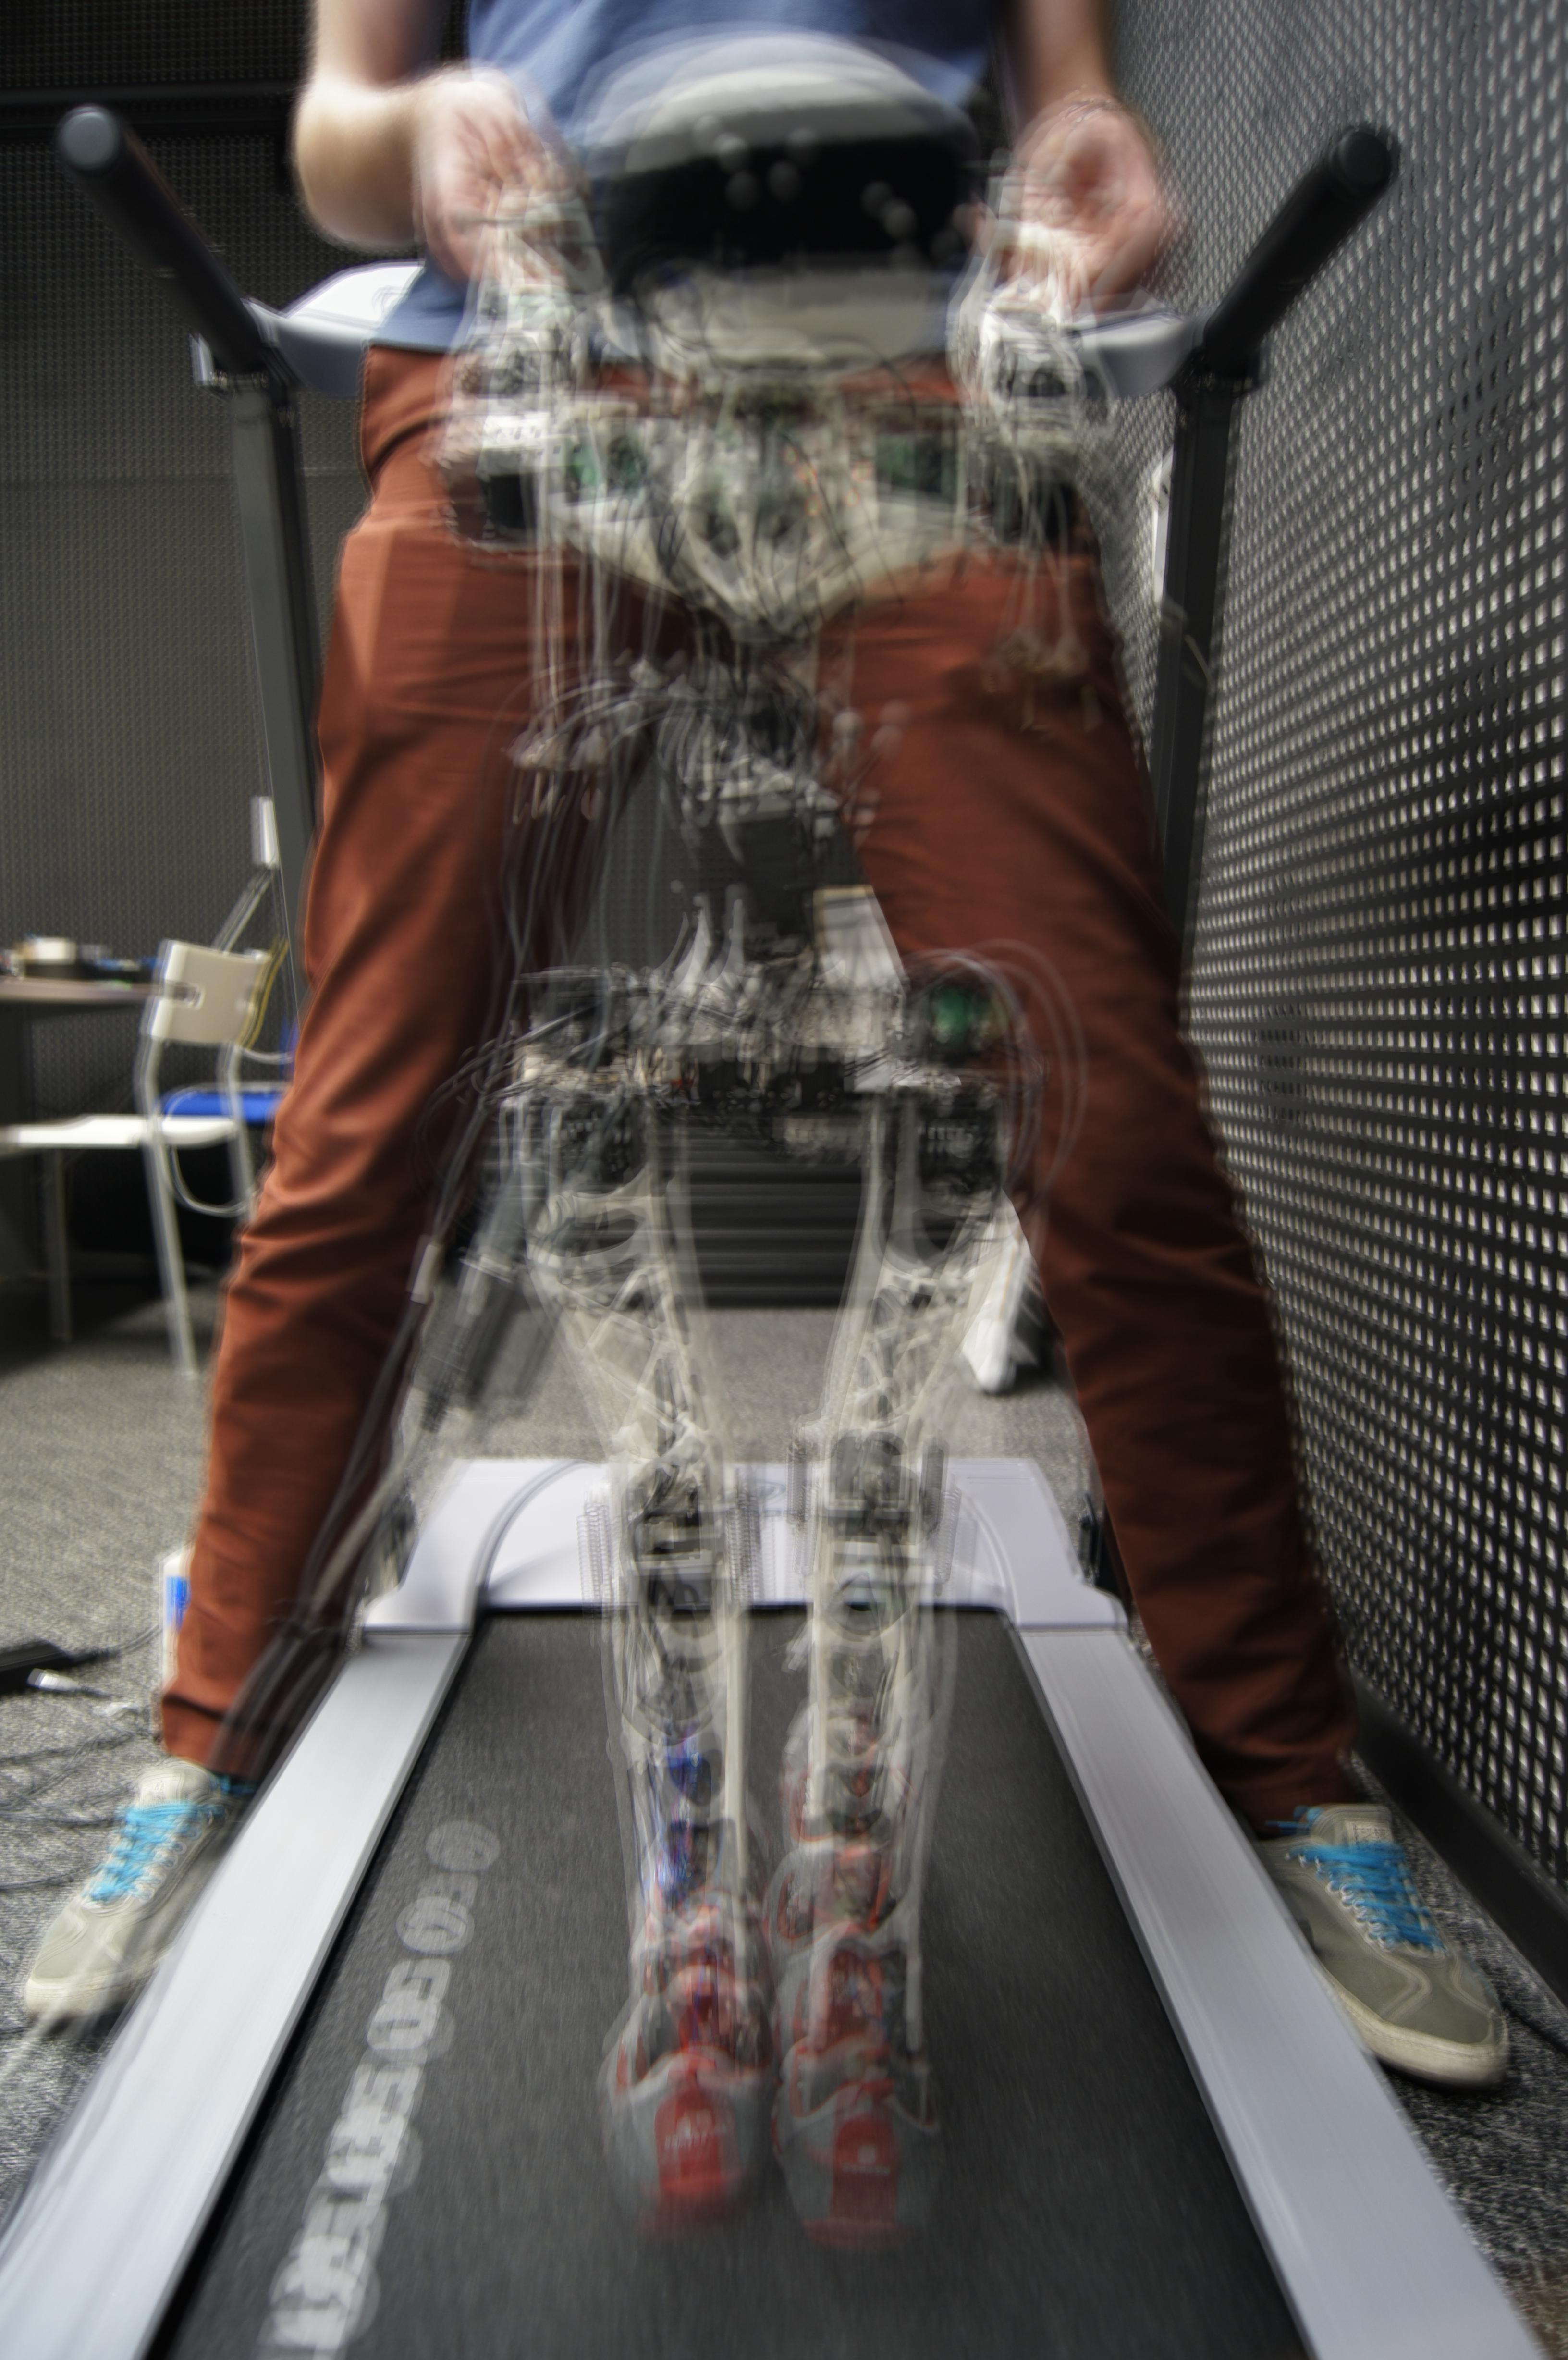
\includegraphics[width=0.4\linewidth]{marche_bended.jpg}}
    \hfil
    \subfloat[][straight thigh]{\label{fig:poppy_walking_straight}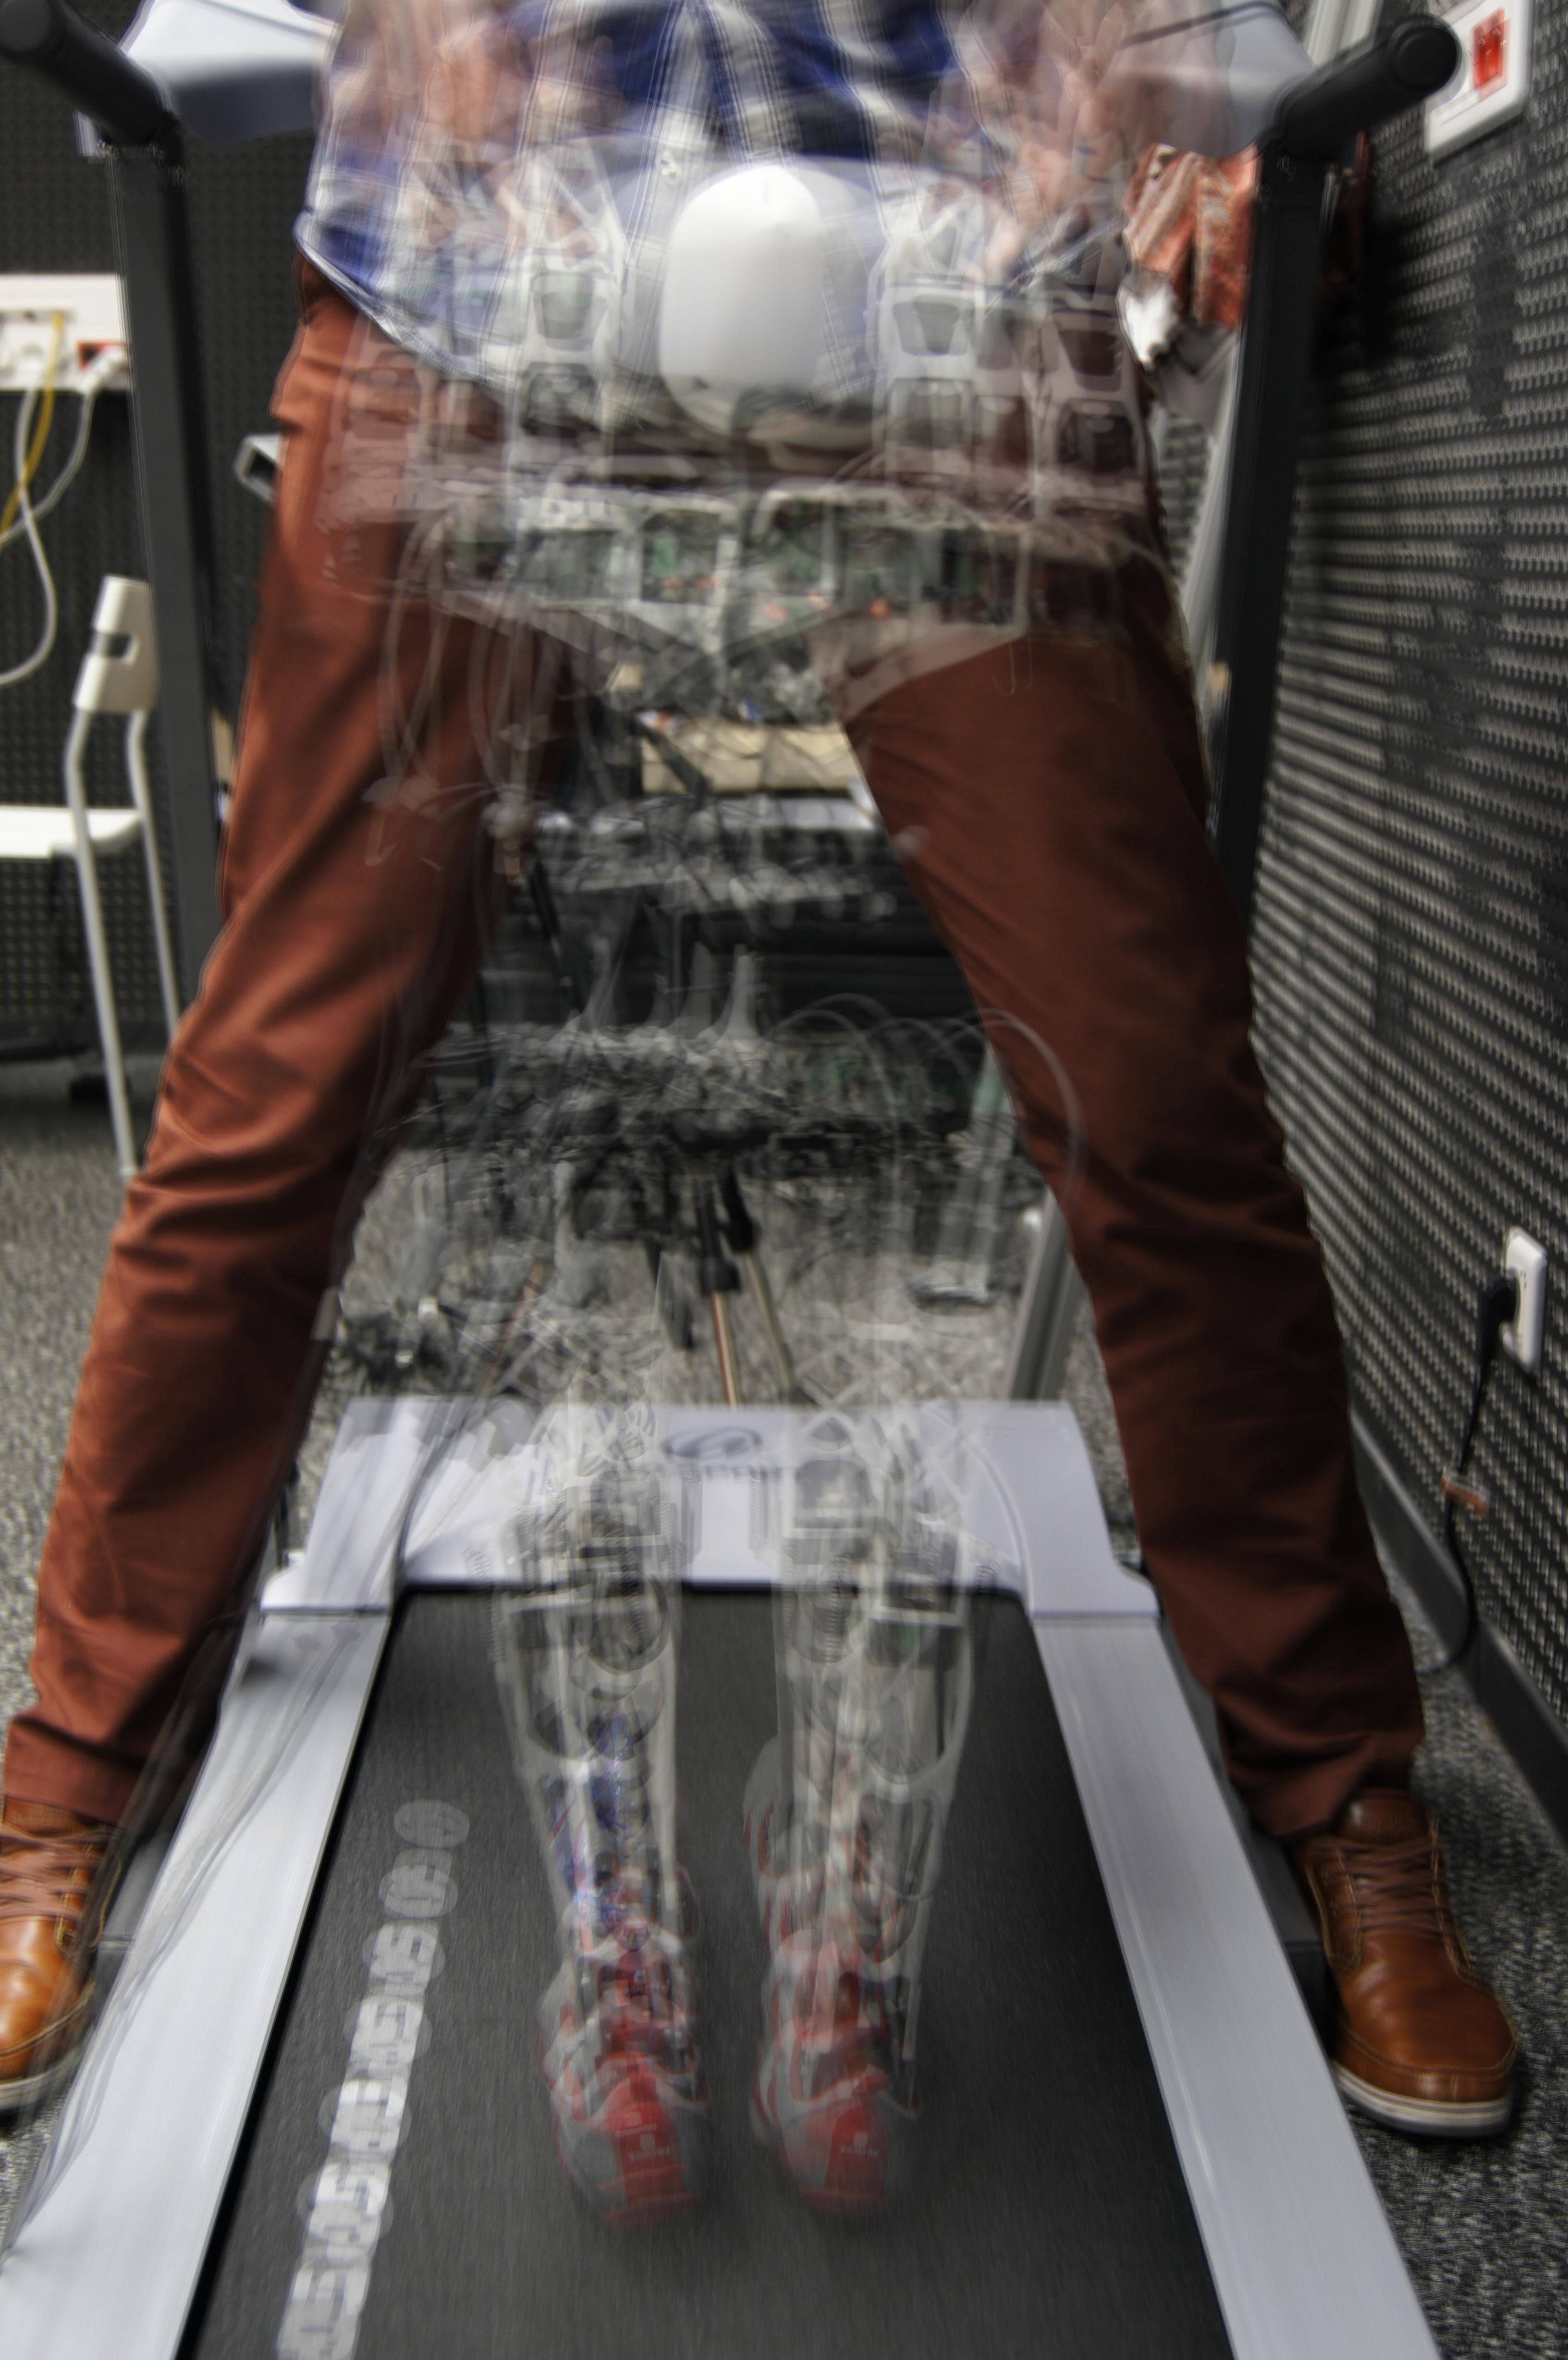
\includegraphics[width=0.4\linewidth]{marche_straight.jpg}}
    \caption{Five pictures have been taken while Poppy was walking and were stacked to obtain a qualitative view of the difference in the walking behavior in function of the morphology of the thigh.}
    \label{fig:poppy_walking_compared}
\end{figure}


\subsection{Conclusion on the thigh shape role for biped locomotion} % (fold)
We focus on the shape of the Poppy thigh and its effect on the robot dynamic. We studied the role of the morphology in the reduction and simplification of the control needed to performs complex task such as biped walking. We have presented the simple theoretical model we used for the design of Poppy thigh based on the inverse pendulum dynamic. We have conducted experiments to evaluate the improvements of the bended thigh on the real robot dynamic and compare it with the model. Thanks to the conception of Poppy allowing easy, cheap and fast morphology modifications, we were able to try another thigh design. We also use a pair of straight thighs which is a more classical approach in humanoid conception. The experimental comparison of the two thighs design confirmed the theoretical results, the bio-inspired thigh design improves Poppy dynamic on two main points useful for biped walking:
\begin{itemize}
    \item It reduces the falling velocity by almost 60\% when the robot is on one foot (single support phase).
    \item It reduces by 30\% the lateral motion needed to transfer the mass of the robot from one foot to the other (double support phase).
\end{itemize}
It is really interesting to note that such a small modification of the robot morphology has a very significant impact on the robot behavior.

These results are interesting but they do not reflect the actual Poppy dynamic while it is walking. To evaluate the effect of the bended thigh on the biped locomotion, we conducted a third experiment where Poppy is walking on a treadmill. In this experiment, we show that the bended thigh has an effect on a complex dynamic task such as the biped locomotion: it reduces the motion amplitude on the upper body of 45\% and increase the head stability of 30\%. We choose these metrics due to our experimental constraints (fixed speed, social guidance) as a qualitative evaluation of the walking gait. Moreover it provides us with an intuitive, yet incomplete evaluation of the walking. Many other measures could have been chosen or combined such as speed, energy consumption or robustness to external perturbations. It is still complicated to understand which metric is the most adapted for the robotic biped locomotion. As human being is trained to recognize biped gait, users can provide guidance to the robot for both safety of exploration and evaluation of the walking behavior.


% subsection Results (end)
